\begin{table}[tb]
  \small
  \centering
  \caption{Comparison of action recognition results with unsupervised learning approaches on NTU 60 dataset. $^\dag$ indicates that results reproduced on our settings of feature dimension size.}
  \begin{tabular}{l|c|c|c}
    \toprule
    % \hline
    Models&Architecture&xview&xsub\\
    \midrule
    \rowcolor{gray!10} \multicolumn{4}{l}{\textit{Single-stream:}}\\
    LongT GAN~\cite{zheng2018unsupervised} & GRU & 48.1 & 39.1\\
    MS$^2$L~\cite{lin2020ms2l} & GRU & - & 52.5\\
    AS-CAL~\cite{rao2021augmented} & LSTM & 64.8 & 58.5 \\
    P$\&$C~\cite{su2020predict} & GRU & 59.3 & 56.1 \\
    SeBiReNet~\cite{nie2020unsupervised} & SeBiReNet & 79.7 & -\\
    ISC~\cite{thoker2021skeleton}& GCN $\&$ GRU & 78.6 & 76.3 \\
    AimCLR~\cite{guo2021contrastive}& GCN & 79.7 & 74.3\\
    CMD$^\dag$~\cite{mao2022cmd} & GRU & 81.3 & 76.8 \\
    GL-Transformer~\cite{kim2022global} & Transformer & 83.8 & 76.3\\
    CPM~\cite{zhang2022contrastive} & GCN & 84.9 & 78.7\\
    \textbf{ActCLR} & GCN & \textbf{86.7} &\textbf{80.9}\\
    \midrule
    \rowcolor{gray!10} \multicolumn{4}{l}{\textit{Three-stream:}}\\
    3s-Colorization~\cite{yang2021skeleton} & DGCNN & 83.1 & 75.2 \\
    3s-CrosSCLR~\cite{li20213d} & GCN & 83.4 & 77.8\\
    3s-AimCLR~\cite{guo2021contrastive}& GCN & 83.8 & 78.9\\
    3s-CMD$^\dag$~\cite{mao2022cmd} & GRU & 85.0 & 79.9 \\
    3s-SkeleMixCLR~\cite{chen2022contrastive} & GCN & 87.1 & 82.7\\
    3s-CPM~\cite{zhang2022contrastive} & GCN & 87.0 & 83.2\\
    \textbf{3s-ActCLR} & GCN & \textbf{88.8} &\textbf{84.3}\\
    \bottomrule
  \end{tabular}
  \label{tab:unsupervised_ntu_60}
\end{table}

% \begin{table*}[tb]
%   \caption{Comparison of action recognition results with unsupervised learning approaches on NTU 120 dataset.}
%   \label{tab:unsupervised_ntu}
%   \centering
%   \begin{tabular}{l|c|c|c|c}
%     \toprule
%     % \hline
%     Models&NTU 60 xview&NTU 60 xsub&NTU 120 xset&NTU 120 xsub\\
%     \midrule
%     MS$^2$L~\cite{lin2020ms2l} & - & 52.5 & - & -\\
%     AS-CAL~\cite{rao2021augmented} & 64.8 & 58.5 & 49.2 & 48.6 \\
%     P$\&$C~\cite{su2020predict} & 59.3 & 56.1 & 44.1 & 41.4 \\
%     SeBiReNet~\cite{nie2020unsupervised} & 79.7 & - & - & -\\
%     AimCLR~\cite{guo2021contrastive} & 79.7 & 74.3 & - & -\\
%     3s-Colorization~\cite{yang2021skeleton} & 83.1 & 75.2 & - & -\\
%     ISC~\cite{thoker2021skeleton} & 78.6 & 76.3 & \textbf{67.1} & \textbf{67.9}\\
%     3s-CrosSCLR~\cite{li20213d} & 83.4 & \textbf{77.8} & 66.7 & \textbf{67.9}\\
%     BCLR & \textbf{83.9} &\textbf{77.8}&66.8& 67.5\\
%     \bottomrule
% \end{tabular}
% \end{table*}
\section{Experiment Results}

For evaluation, we conduct our experiments on the following two datasets: the NTU RGB+D dataset~\cite{shahroudy2016ntu,liu2019ntu} and the PKUMMD dataset~\cite{liu2020pku}. 
% Our goal is to obtain the feature encoder $f(\cdot)$ which can generate good feature representations for action recognition. 

\subsection{Datasets and Settings}
\noindent$\bullet$ \textbf{NTU RGB+D Dataset 60 (NTU 60)}~\cite{shahroudy2016ntu} is a large-scale dataset which contains 56,578 videos with 60 action labels and 25 joints for each body, including interactions with pairs and individual activities.

\vspace{1mm}

\noindent$\bullet$ \textbf{NTU RGB+D Dataset 120 (NTU 120)}~\cite{liu2019ntu} is an extension to NTU 60 and the largest dataset for action recognition, which contains 114,480 videos with 120 action labels. Actions are captured with 106 subjects with multiple settings using 32 different setups.


\vspace{1mm}

\noindent$\bullet$ \textbf{PKU Multi-Modality Dataset (PKUMMD)}~\cite{liu2020pku} covers a multi-modality 3D understanding of human actions. The actions are organized into 52 categories and include almost 20,000 instances. There are 25 joints in each sample. The PKUMMD is divided into part I and part II. Part II provides more challenging data, because the large view variation causes more skeleton noise.

To train the network, all the skeleton sequences are temporally down-sampled to 50 frames. The encoder $f(\cdot)$ is based on ST-GCN~\cite{yan2018spatial} with hidden channels of size 16, which is a quarter the size of the original model. The projection heads for contrastive learning and auxiliary tasks are all multilayer perceptrons, projecting features from 256 dimensions to 128 dimensions. $\tau_q$ is $0.1$ and $\tau_k$ is $0.04$. We employ a fully connected layer $\phi(\cdot)$ for evaluation.

\begin{table}[tb]
  \small
  \centering
  \caption{Comparison of action recognition results with unsupervised learning approaches on NTU 120 dataset. $^\dag$ indicates that results reproduced on our settings of feature dimension size.}
  \begin{tabular}{l|c|c|c}
    \toprule
    % \hline
    Models&Architecture&xset&xsub\\
    \midrule
    \rowcolor{gray!10} \multicolumn{4}{l}{\textit{Single-stream:}}\\
    AS-CAL~\cite{rao2021augmented} & LSTM & 49.2 & 48.6 \\
    AimCLR~\cite{guo2021contrastive} & GCN & 63.4 & 63.4\\
    CMD$^\dag$~\cite{mao2022cmd} & GRU & 66.0 & 65.4 \\
    GL-Transformer~\cite{kim2022global} & Transformer & 68.7 & 66.0\\
    CPM~\cite{zhang2022contrastive} & GCN & 69.6 & 68.7\\
    \textbf{ActCLR} & GCN & \textbf{70.5} &\textbf{69.0}\\
    \midrule
    \rowcolor{gray!10} \multicolumn{4}{l}{\textit{Three-stream:}}\\
    3s-CrosSCLR~\cite{li20213d} & GCN & 66.7 & 67.9\\
    3s-AimCLR~\cite{guo2021contrastive} & GCN & 68.8 & 68.2\\
    3s-CMD$^\dag$~\cite{mao2022cmd} & GRU & 69.6 & 69.1 \\
    3s-SkeleMixCLR~\cite{chen2022contrastive} & GCN & 70.7 & 70.5\\
    3s-CPM~\cite{zhang2022contrastive} & GCN & 74.0 & 73.0\\
    \textbf{3s-ActCLR} & GCN & \textbf{75.7} &\textbf{74.3}\\
    \bottomrule
  \end{tabular}
  \label{tab:unsupervised_ntu_120}
\end{table}

To optimize our network, Adam optimizer~\cite{newey1988adaptive} is applied, and we train the network on one NVIDIA TitanX GPU with a batch size of 128 for 300 epochs.



\section{Preliminaries of NeRF}\label{sec:priliminary}
The 3D scene can be represented with the NeRF model, and the neural network is utilized to map a point position $\boldsymbol{x} \in \mathbb{R}^3$  and a view direction $\boldsymbol{d} \in \mathbb{R}^3$ to the corresponding color $\boldsymbol{c} \in \mathbb{R}^3$ and volume density $\sigma$ \cite{mildenhall2020nerf}.  We apply the voxel grid to represent the scene considering the low computational cost of voxel-based NeRF \cite{sun2021direct}. The density voxel grid $\boldsymbol{V}_{\text{density}}$  and  feature voxel grid $\boldsymbol{V}_{\text{color}}$  with a shallow MLP  are adopted to represent the scene geometry and appearance, respectively. Given input queries $\boldsymbol{x} $ and $\boldsymbol{d} $,  the outputs are obtained with the interpolation
\begin{equation}
\begin{aligned}
 \sigma &= \text{inter}(\boldsymbol{x}, \boldsymbol{V}_{\text{density}})  \\
 \boldsymbol{c} &= \text{MLP}_{\theta}(\text{inter}(\boldsymbol{x}, \boldsymbol{V}_{\text{color}}), \boldsymbol{x} , \boldsymbol{d}) 
  \label{eq:important}
  \end{aligned}
\end{equation}
To render the image, the pixel color $\boldsymbol{C}(\boldsymbol{r})$ along the camera ray $\boldsymbol{r}(t) = \boldsymbol{r_0}+ t \boldsymbol{d}$ is approximated by the volume rendering
\begin{equation}
\boldsymbol{C}(\mathbf{r})=\int_{t_1}^{t_2} T(t) \sigma(\boldsymbol{r}(t)) \mathbf{c}(\boldsymbol{r}(t), \mathbf{d}) d t,
\end{equation}
where  $t_1$ and $t_2$ are near and far bounds for sampling points, $\boldsymbol{r_0}$ is the camera origin, and $T(t)$ is accumulated transmittance along the ray from $t_1$ to $t$ defined by
\begin{equation}
T(t)=\exp \left(-\int_{t_1}^t \sigma(\boldsymbol{r}(s)) d s\right).
\label{eq:transmittance}
\end{equation}
The NeRF model is trained by minimizing the  loss between the rendered pixel color $\boldsymbol{C}(\boldsymbol{r})$ and observed pixel color $\hat{\boldsymbol{C}}(\boldsymbol{r})$given by
\begin{equation}
\mathcal{L}_{\text {Color }}=\sum_{\boldsymbol{r} \in \mathcal{R}(\mathbf{P})}\|\hat{\boldsymbol{C}}(\boldsymbol{r})-\boldsymbol{C}(\boldsymbol{r})\|_2^2,
\end{equation}
where $\mathcal{R}(\mathbf{P})$ is the set of rendered rays in a batch.


\section{Implementation Detail of Detectors}
For FCOS3D, we utilize a ResNet-101-DCN\cite{he2016deep, dai2017deformable} as the backbone. The model is trained for 24 epochs using the SGD optimizer with an initial learning rate of 1e-4 and a momentum of 0.9. We set the weight decay to 1e-5, and the max norm of gradient clipping to 35. We also adopt a step decay learning rate scheduler with a 0.1$\times$ decrease at epoch 20 and 23, along with 1000 iterations of linear warm-up. For SMOKE, we employ a DLA-34\cite{yu2018deep} as the backbone. We use the Adam optimizer with an initial learning rate 1e-4, and the remaining settings are the same as FCOS3D. For both detectors, their backbones are initialized with ImageNet pre-trained weights. The batch size for training is set to 16.





\setlength{\tabcolsep}{8.5pt}
\begin{table}[t]
  \small
  \begin{center}
  \begin{tabular}{@{}ccccc@{}}
    \toprule
     3DAug  & DS & LET-AP &  LET-APH & LET-APL \\
    \midrule
      -     &  -           &  0.585 & 0.573 & 0.393 \\
     \checkmark  & - & 0.584 & 0.572   & 0.394 \\
    \checkmark & \checkmark &  \textbf{0.590} & \textbf{0.578} & \textbf{0.403} \\
    \bottomrule
  \end{tabular}
  \end{center}
  \caption{\textbf{Ablation Study} of Drive-3DAug for FCOS3D on Waymo validation set. 3DAug means we use DVGO \cite{sun2021direct} for data augmentation. DS means depth supervision.}
  \label{tab:ablation_depth}
\end{table}


\begin{figure}[t]
    \begin{center}
        \includegraphics[width=0.99\linewidth]{fig/depth_v1.pdf}
    \end{center}
    \caption{\textbf{Visualization of rendered depth map.}  The model with depth supervision depicts better performance.}
    \label{fig:depth}
\end{figure}



\section{Ablation Study on Depth Supervision.}
We qualitatively and quantitatively investigate the effect of depth supervision on background model training and 3D augmentation.
Table~\ref{tab:ablation_depth} shows that the 3D augmentation based on background model trained with depth supervision has better performance, with LET-AP (0.590 vs 0.585).
Figure~\ref{fig:depth} shows that NeRF can reconstruct the background with high quality given depth supervision, and the 3D background model quality can be decreased without depth information.
Thus, LET-AP, LET-APH and LET-APL on car have a slight decrease with 0.001 for 3D augmentation using background model without supervision.





\section{Visualization of Drive-3DAug}
% \tww{Aug car, person, cyclist, including RGB and depths map}
% We visualize the reconstructed depth map and new driving scene generated by Drive-3DAug in Figure~\ref{fig:depth}, indicating that 
We augment car in Figure~\ref{fig:more_vis}, indicating that
we can generate scene with high quality with Drive-3DAug.
Compared with car, pedestrian and cyclist are not rigid body and the size is small, not well applicable for NeRF modelling.
We model pedestrian and cyclist as rigid boby in the present study, which can cause the decay of object model performance.
As shown in Figure~\ref{fig:person}, although there exists flaw for augmented 
pedestrian and cyclist, we can still augment them to improve the detector performance.



\section{Cross-dataset Drive-3DAug}
We have reconstructed thousands of background and object models in Waymo and nuScenes dataset.
These models can serve as the general model assets, convenient for creating new driving scenes inside a specific dataset or cross different datasets.
As shown in Figure \ref{fig:cross}, we compose the object models from nuScenes and the background models from Waymo to create new driving scenes. This can further enlarge the diversity of the training data, and we can generate large amounts of data for the study of model generalization across different datasets.


\begin{figure*}[t]
    \begin{center}
\includegraphics[width=0.9\linewidth]{fig/more_aug.pdf}
    \end{center}
    \caption{\textbf{Visualization of the generated images by Drive-3DAug.} The yellow boxes indicate the newly added cars for the background.}
    \label{fig:more_vis}
\end{figure*}

\begin{figure*}[t]
    \begin{center}
        \includegraphics[width=0.9\linewidth]{fig/person.pdf}
    \end{center}
    \caption{\textbf{Visualization of the generated images by Drive-3DAug.} The yellow and red boxes indicate the augmented pedestrian and cyclist, respectively.}
    \label{fig:person}
\end{figure*}



\begin{figure*}[t]
    \begin{center}
        \includegraphics[width=0.9\linewidth]{fig/cross.pdf}
    \end{center}
    \caption{\textbf{Image Generation cross datasets.} We place the cars from nuScenes on the backgrounds of Waymo. The yellow boxes indicate the augmented cars.}
    \label{fig:cross}
\end{figure*}




\subsection{Evaluation and Comparison}
To make a comprehensive evaluation, we compare our method with other methods under variable settings.
\vspace{1mm}

\pgfplotsset{compat=1.17}

\pgfplotstableread{
     Answer   Count   
     Yes 8
     Questioning 3
     No 29
     Other 3
}{\mytableorgtrans}

\pgfplotstableread{
     Answer   Count   
     Yes 3
     Questioning 4
     No 39
}{\mytablescholtrans}

\pgfplotstableread{
     Answer 2018 2019 2020 {2021--2022}
     Yes 5 8 17 51
     Questioning 3 0 3 17
     No 48 84 98 186
}{\mytablecommtrans}

\begin{figure}[t]
\centering
\subfloat[Queer in AI Community: Are you Trans?] {
    \begin{tikzpicture}[trim axis left]
      \pgfplotsset{
          scale only axis
      }
        \begin{axis} [
            width=4cm, height=3cm,
            enlarge x limits={abs=0.5cm},
            ybar=0, bar width=5pt,
            ymin=0, ymax=200,
            xtick=data,
            ticklabel style = {font=\footnotesize},
            symbolic x coords={Yes, Questioning, No},
            xticklabel style={rotate=45,anchor=north east,inner sep=0mm},
            xtick style={draw=none},
            ylabel={Number of respondents}, ylabel near ticks,
            label style = {font=\footnotesize},
            ymajorgrids=true,
            legend style={at={(0.02,0.98)},anchor=north west, nodes={scale=0.75}},
            legend cell align={left}]
        \addplot [mycolor1!60!black, fill=mycolor1] table [x=Answer,y=2018] {\mytablecommtrans};
        \addplot [mycolor2!60!black, fill=mycolor2] table [x=Answer,y=2019] {\mytablecommtrans};
        \addplot [mycolor3!60!black, fill=mycolor3] table [x=Answer,y=2020] {\mytablecommtrans};
        \addplot [mycolor4!60!black, fill=mycolor4] table [x=Answer,y={2021--2022}] {\mytablecommtrans};
        \legend{2018, 2019, 2020, {2021--2022}}
        \addplot [only marks, mark=asterisk, mark size=1pt] table[row sep=\\] {
            x y\\
            [normalized]0.83 10\\
            [normalized]1.04 10\\
        };
        \end{axis} 
    \label{fig:org_trans_c}
    \end{tikzpicture}
}\hspace{1cm}
\subfloat[Queer in AI Organizers: Are you Trans?] {
    \begin{tikzpicture}[trim axis left]
      \pgfplotsset{
          scale only axis
      }
        \begin{axis} [
            width=3.5cm, height=3cm,
            ybar, bar width=10pt,
            enlarge x limits={abs=0.75cm},
            ymin=0, ymax=45,
            xtick=data,
            ticklabel style = {font=\footnotesize},
            symbolic x coords={Yes,Questioning,No,Other},
            xticklabel style={rotate=45,anchor=north east,inner sep=0mm},
            xtick style={draw=none},
            ylabel={Number of respondents}, ylabel near ticks,
            label style = {font=\footnotesize},
            ymajorgrids=true]
        \addplot [mycolor1!60!black, fill=mycolor1] table [x=Answer,y=Count] {\mytableorgtrans};
        \addplot [only marks, mark=asterisk, mark size=1pt] table[row sep=\\] {
            x y\\
            Questioning 5\\
            Other 5\\
        };
        \end{axis} 
    \label{fig:org_trans_o}
    \end{tikzpicture}
}\hspace{1cm}
\subfloat[Queer in AI Scholarship Recipients: Are you Trans?] {
    \begin{tikzpicture}[trim axis left]
      \pgfplotsset{
          scale only axis
      }
        \begin{axis} [
            width=3cm, height=3cm,
            ybar, bar width=10pt,
            enlarge x limits={abs=0.75cm},
            ymin=0, ymax=45,
            xtick=data,
            ticklabel style = {font=\footnotesize},
            symbolic x coords={Yes,Questioning,No},
            xticklabel style={rotate=45,anchor=north east,inner sep=0mm},
            xtick style={draw=none},
            ylabel={Number of respondents}, ylabel near ticks,
            label style = {font=\footnotesize},
            ymajorgrids=true]
        \addplot [mycolor1!60!black, fill=mycolor1] table [x=Answer,y=Count] {\mytablescholtrans};
        \addplot [only marks, mark=asterisk, mark size=1pt] table[row sep=\\] {
            x y\\
            Yes 5\\
        };
        \end{axis} 
    \label{fig:org_trans_sr}
    \end{tikzpicture}
  }
\caption{Queer in AI's statistics for transgender community members (\subref{fig:org_trans_c}), organizers (\subref{fig:org_trans_o}), and scholarship recipients (\subref{fig:org_trans_sr}) respectively. Write-in responses were aggregated by a team of Queer in AI organizers. For categories with $\leq3$ responses (marked by *), exact numbers are omitted to protect anonymity. \label{fig:trans}}
\end{figure}

\noindent\textbf{1) Linear Evaluation.}
In the linear evaluation mechanism, a linear classifier $\phi(\cdot)$ is applied to the fixed encoder $f(\cdot)$ to classify the extracted features. We adopt action recognition accuracy as a measurement. Note that this encoder $f(\cdot)$ is fixed in the linear evaluation protocol.

Compared with other methods in Tables~\ref{tab:unsupervised_ntu},~\ref{tab:unsupervised_ntu_60} and~\ref{tab:unsupervised_ntu_120}, our model shows superiority on these datasets. We find that the transformation that 3s-CrosSCLR~\cite{li20213d} and 3s-AimCLR~\cite{guo2021contrastive} design in the contrastive learning task is unified for different regions, which makes the data transformation interfere with the motion information. On the contrary, our method adopts MATS for semantic-aware motion-adaptive data transformation. Thus, the features extracted by our method maintain better action information which is more suitable for downstream tasks. 

\vspace{1mm}


\noindent\textbf{2) Supervised Finetuning.}
We first pretrain the encoder $f(\cdot)$ in the self-supervised learning setting, and then finetune the entire network. We train the encoder $f(\cdot)$ and classifier $\phi(\cdot)$ using complete training data.

Table~\ref{tab:supervised_ntu} displays the action recognition accuracy on the NTU datasets. This result confirms that our method extracts the information demanded by downstream tasks and can better benefit action recognition. 
In comparison with state-of-the-art supervised learning methods, our model achieves better performance.

\vspace{1mm}

% \noindent\textbf{\wh{3)} Semi-Supervised Approaches.}
% In semi-supervised learning, the training process utilizes both labeled data and unlabeled data. Generally, the encoder $f(\cdot)$ is pretrained with the contrastive learning task with full data, and then fine-tuned with the classifier $\phi(\cdot)$ with labeled data. To give a comprehensive and thorough evaluation, we conduct experiments under different settings, including $1\%$, $5\%$, $10\%$ and $20\%$ of labeled skeleton sequences. We also show the comparison results with the state-of-the-art methods. 

% In Table~\ref{tab:semi_supervised_pku} and~\ref{tab:semi_supervised_ntu}, we notice that with small subsets of the datasets, our method improves the accuracy considerably and performs better than the state-of-the-art methods. Especially with smaller training data, our method outperforms the state-of-the-art by large margins.

% \noindent\textbf{\wh{3)} Parameter-Efficient Finetuning.}
% We also first pretrain the encoder $f(\cdot)$, and after self-distillating the encoder $f(\cdot)$, employ the gradient-guided parameter-efficient finetuning.

% Table~\ref{tab:supervised_ntu} shows the action recognition accuracy on the NTU datasets. Our method achieves comparable performance to full model fine-tuning with fewer trainable parameters. Moreover, we can adjust the \wh{number} of parameters that need to be finetuned through the threshold, which makes the finetuning more controllable, as shown in Table~\ref{tab:effi}.

\vspace{1mm}

\noindent\textbf{3) Transfer Learning.} 
To explore the generalization ability, we evaluate the performance of transfer learning. In transfer learning, we exploit self-supervised task pretraining on the source data. Then we utilize the linear evaluation mechanism to evaluate on the target dataset. In linear evaluation, the encoder $f(\cdot)$ has fixed parameters without fine-tuning.

As shown in Table~\ref{tab:trans_pku}, our method achieves significant performance. Our method employs MATS to remove irrelevant information, and SAFP to retain information related to downstream tasks. This allows our encoder $f(\cdot)$ to obtain stronger generalization performance.

\vspace{1mm}

\noindent\textbf{4) Unsupervised Action Segmentation.} 
To explore the extraction of local features by our method, we used unsupervised action segmentation as an evaluation metric. We pre-train the encoder $f(\cdot)$ on the NTU 60 dataset. Then we utilize the linear evaluation mechanism to evaluate \wh{the results} on the PKUMMD dataset. In linear evaluation, the encoder $f(\cdot)$ has fixed parameters without fine-tuning.

As shown in Table~\ref{tab:seg_pkuII}, our method achieves significant performance. Because our method focuses on the main occurrence region of the action, it is possible to locate the actions out of the long sequence.

\begin{table}[tb]
\small
\begin{center}
\caption{Comparison of the action segmentation performance on PKUMMD II xview dataset with linear evaluation pretrained on NTU 60 xview dataset.}
\label{tab:seg_pkuII}
\begin{tabular}{l|c|c|c|c|c}
\toprule
\multirow{2.5}*{Models}&\multirow{2.5}*{Stream}&\multicolumn{4}{c}{PKUMMD II xview}\\
\cmidrule(lr){3-6}
&&ACC & MACC & FWIoU & mIoU\\
\midrule
AimCLR~\cite{guo2021contrastive} & joint & 39.77 & 28.68 & 26.79 & 15.67\\
\textbf{ActCLR} & joint & \textbf{51.29}  & \textbf{31.97} & \textbf{35.24} & \textbf{21.38}\\
\midrule
AimCLR~\cite{guo2021contrastive}& motion& 42.32 & 26.65 & 29.92 & 15.92 \\
\textbf{ActCLR} & motion& \textbf{56.69} & \textbf{39.45} & \textbf{41.34} & \textbf{27.73}\\
\midrule
AimCLR~\cite{guo2021contrastive}& bone& 54.22 & 39.52 & 39.41 & 27.36\\
\textbf{ActCLR} &bone& \textbf{59.09} & \textbf{41.14} & \textbf{41.54} & \textbf{28.89}\\
\bottomrule
\end{tabular}
\end{center}
\end{table}


\subsection{Ablation Study}
Next, we conduct ablation experiments to give a more detailed analysis of our proposed approach.

\vspace{1mm}

\noindent\textbf{1) Analysis of Motion-Adaptive Data Transformation.} 
Data transformation is very important for consistency learning. To explore the influence of motion-adaptive data transformations, we test the action recognition accuracy under different data transformations. 
%
As shown in Table~\ref{tab:data}, the motion-adaptive transformation can obtain better performance than full region (the whole skeleton data) in different noise settings. It is also observed that when the noise strength increases, our performance degradation is much smaller than that of full region. This indicates that the design is more robust to data transformation.
% the consistency of the feature space is further enhanced with actionlet-dependent data transformations. And under stronger data transformations, our method still maintains the motion semantic information. Accordingly, the performance of downstream tasks is improved. 

To explore the influence of different data transformations on the contrastive learning effect, we test the action recognition accuracy under different data transformation combinations. As shown in Table~\ref{tab:com}, the consistency of the feature space is further enhanced with more data transformations. Thus, the performance of the downstream task is improved.

% PTMTorrrent
\newcommand{\numberOfModelHub}{5\xspace}

\newcommand{\TotalNumberOfPackages}{{15,913}\xspace}
% 12401 from Hugging Face
% 185 from ONNX
% 33 from Model Hub
% 3245 from Model Zoo
% 49 from PyTorch Hub
% SUM (by Nick): 15,913

\newcommand{\HFNumberOfPackages}{{12,401}\xspace}
\newcommand{\HFNumberOfPackagesMetadata}{{124,427}\xspace}
\newcommand{\MZNumberOfPackages}{3,245\xspace}
\newcommand{\PHNumberOfPackages}{{49}\xspace}
\newcommand{\MHNumberOfPackages}{{33}\xspace}
\newcommand{\ONNXNumberOfPackages}{{185}\xspace}

\newcommand{\TotalDataSize}{\textasciitilde{61TB}\xspace}
\newcommand{\HFDataSize}{{61TB}\xspace}
\newcommand{\MZDataSize}{{115GB}\xspace}
\newcommand{\PHDataSize}{{1.5GB}\xspace}
\newcommand{\MHDataSize}{{721MB}\xspace}
\newcommand{\ONNXDataSize}{{441MB}\xspace}
%%%



% ICSE submission - HFTorrent v1

\newcommand{\PTMDatasetNPackages}{63,182\xspace}
\newcommand{\PTMDatasetPercentage}{{99.7\%}\xspace}
\newcommand{\PTMDatasetFailedPackages}{{186}\xspace}
\newcommand{\PTMDatasetFailedPercentage}{{0.3\%}\xspace}

\newcommand{\PTMDatasetNReposWithSignedCommits}{{132}\xspace}
\newcommand{\PTMDatasetPercentOfSignedCommits}{{0.208\%}\xspace}


\newcommand{\PercentOfVerifiedOrgs}{{3.188\%}\xspace}
\newcommand{\NOrganizations}{{6,243}\xspace}
\newcommand{\NVerifedOrgs}{{199}\xspace}

\newcommand{\NOfRepositoriesWithMalware}{{1}\xspace}
\newcommand{\PercentageOfRepositoriesWithMalware}{{0.002\%}\xspace}
\newcommand{\TotalRepositoriesForMalwareScanning}{{63,366}\xspace}

\vspace{1mm}

\noindent\textbf{2) Analysis of Semantic-Aware Feature Pooling.} 
To explore the semantic-aware feature pooling, we perform this pooling on different streams. Table~\ref{tab:effi} shows the results of accuracy of action recognition under different settings. We note that better performance is obtained with offline, as it makes offline to generate better positive sample features for contrastive learning. Using this module in online reduces the benefits exposed by the non-actionlet transformation.
% In offline network feature extraction, $\kappa$ controls the attention of the actionlet. A smaller $\kappa$ makes the feature pooling close to the global average pooling, while a larger $\kappa$ makes the features extracted only from the actionlet region.
% %
% Table~\ref{tab:effi} shows the results of different $\kappa$. 
% We notice that using only SAFP can get better performance than using GAP. And the combination of both is used to obtain more informative features.

\begin{table}[tb]
\small
\begin{center}
\caption{Analysis of semantic-aware feature pooling on NTU 60 xview dataset with the joint stream.}
\label{tab:effi}
\begin{tabular}{l|c|c}
\toprule
% \multirow{2.5}*{Proportion}&\multicolumn{2}{|c}{xview}\\
% \cmidrule(lr){2-3}
Modules& KNN & Linear\\
\midrule
w/o SAFP & 76.38 & 85.69\\
% 1.0 & 75.89 & 86.28\\
offline w/ SAFP  & \textbf{78.04} & \textbf{86.79}\\
online w/ SAFP & 76.02 & 85.25\\
online + offline w/ SAFP & 76.71 & 85.92\\
\bottomrule
\end{tabular}
\end{center}
\vspace{-1em}
\end{table}


\vspace{1mm}

% \noindent\textbf{3) Analysis of Unsupervised Actionlet Selection.} 
% We explored the effect of thresholding on actionlet selection for feature learning. As shown in Table~\ref{tab:threshold}, when the threshold is small, many joints are selected causing the actionlet to contain many static regions. When the threshold value is relatively large, the selected area is relatively small, making the motion information lost.
% \begin{table}[tb]
\small
\begin{center}
\caption{Analysis of threshold of unsupervised action selection on NTU 60 xview dataset with the joint stream.}
\label{tab:threshold}
\begin{tabular}{l|c|c}
\toprule
% \multirow{2.5}*{Threshold}&\multicolumn{2}{|c}{xview}\\
% \cmidrule(lr){2-3}
Threshold $k$& KNN & Linear\\
\midrule
0.5 & 77.66	& 86.44\\
1.0 & \textbf{78.04} & \textbf{86.79}\\
2.0 & 76.28 & 85.66 \\
\bottomrule
\end{tabular}
\end{center}
\end{table}

% \vspace{1mm}

\noindent\textbf{3) Analysis of Actionlet and Non-Actionlet Semantic Decoupling.}   
In Fig.~\ref{fig:acc}, we show the performance of extracting only actionlet region information and non-actionlet region information for action recognition. The accuracy of the actionlet region for action recognition is comparable to the accuracy of the whole skeleton data. In contrast, the performance of the features of non-actionlet regions for action recognition is much lower. This shows that the actionlet area does contain the main motion information. 
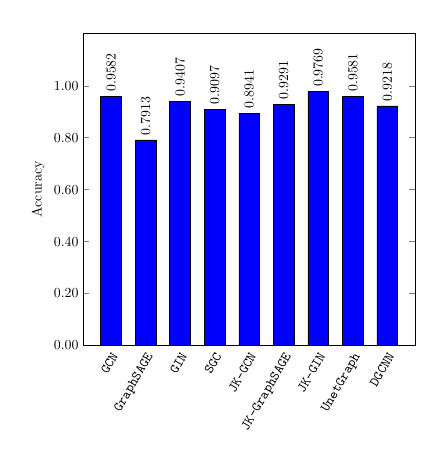
\begin{tikzpicture}[scale=0.5, every node/.style={scale=1.0}]
    \begin{axis}[
        width  = 0.825*\textwidth,
        height = 9.5cm,
        ymin=0.0,ymax=1.2,
        ytick={0,0.2,0.4,0.6,0.8,1.0},
        major x tick style = transparent,
        ybar=5*\pgflinewidth,
        bar width=15.0pt,
%        ymajorgrids = true,
%        xlabel = {Model},
        ylabel = {Accuracy},
        symbolic x coords={
MLP,
WL-Kernel,
Feather,
Slaq-LSD,
Slaq-VGNE,
GCN,
GraphSAGE,
GIN,
SGC,
JK-GCN,
JK-GraphSAGE,
JK-GIN,
UnetGraph,
DGCNN
},
        xtick=data,
	y tick label style={
%		rotate=90,
    		/pgf/number format/.cd,
   		fixed,
   		fixed zerofill,
    		precision=2},
%	yticklabel pos=right,
%        xtick = data,
        x tick label style={
        		rotate=60,
		font=\tt,
		anchor=north east,
		inner sep=0mm
		},
%		font=\small},
%        scaled y ticks = false,
	%%%%% numbers on bars and rotated
        nodes near coords,
        every node near coord/.append style={rotate=90, 
        								   anchor=west,
%								   font=\footnotesize,
								   /pgf/number format/.cd,
								   	fixed zerofill,
									precision=4
								   },
        %%%%%
%        enlarge x limits=0.03,
        enlarge x limits=0.1,
%        enlarge x limits=0.25,
        legend cell align=left,
        legend pos=south east,
%        legend style={
%                at={(1,1.05)},
%                anchor=south east,
%	        nodes={rotate=90},%%%%% rotate text in legend
%                at={(0.125,0)},
%                at={(0.125,0)},
%                at={(0.8775,0)},
%                at={(0.89,0.02)},
%                anchor=south,
%                column sep=1ex
%        },
%        axis x line*=bottom
    ]
%\addplot[fill=red,opacity=1.00]
%coordinates {
%(MLP,0.8054)
%(WL-Kernel,0.7053)
%(Feather,0.8488)
%(Slaq-LSD,0.7799)
%(Slaq-VGNE,0.5499)
%};
\addplot[fill=blue,opacity=1.00]
coordinates {
(GCN,0.9582)
(GraphSAGE,0.7913)
(GIN,0.94070)
(SGC,0.9097)
(JK-GCN,0.8941)
(JK-GraphSAGE,0.9291)
(JK-GIN,0.9769)
(UnetGraph,0.9581)
(DGCNN,0.9218)
};
\end{axis}
\end{tikzpicture}


\vspace{1mm}

\noindent\textbf{4) Visualization of Average Motion and Actionlet.} 
\wh{Fig}.~\ref{fig:mean} shows a visualization of the average motion and actionlet respectively. The average motion has no significant motion information and serves as a background. The actionlet, shown in Fig.~\ref{fig:act}, selects the joints where the motion mainly occurs. Our actionlet is spatio-temporal, because the joints with motion may change when the action is performed.
\input{fig/mean.tex}